\documentclass[onecolumn]{IEEEtran}

\usepackage[left=1.5cm,right=1.5cm]{geometry}
\usepackage[
spanish,
es-nodecimaldot,
es-tabla
%english
]{babel}
\usepackage[utf8]{inputenc}
\usepackage[T1]{fontenc}
\usepackage{float}
\usepackage{crossreftools}
\usepackage{graphicx}
\usepackage{grffile}
\usepackage{longtable}
\usepackage{wrapfig}
\usepackage{rotating}
\usepackage[normalem]{ulem}
\usepackage{amsmath}
\usepackage{textcomp}
\usepackage{amssymb}
\usepackage{capt-of}
\usepackage{hyperref}
\usepackage{minted}
\usepackage{subfiles}
\usepackage{caption}
\usepackage{subcaption}
\usepackage[acronym, toc]{glossaries}

\usepackage{fancyhdr}
\usepackage{graphicx}
\usepackage[table,xcdraw]{xcolor}
\usepackage{multicol}
\usepackage{tabularx,booktabs}
\usepackage{siunitx}

\usepackage{grffile}
\usepackage{longtable}
\usepackage{wrapfig}
\usepackage{rotating}
\usepackage[normalem]{ulem}
\usepackage{amsmath}
\usepackage{textcomp}
\usepackage{amssymb}
\usepackage{capt-of}
\usepackage{booktabs}
\usepackage{hyperref}
\usepackage{caption}

\definecolor{LightGray}{gray}{0.9}
\definecolor{DarkGray}{HTML}{191919}
\definecolor{custom}{HTML}{F8F8F8}

\newenvironment{code}{\captionsetup{type=listing}}{}

\usemintedstyle{emacs}

\usepackage[ruled,vlined]{algorithm2e}


\renewcommand{\listingscaption}{Código}
\renewcommand\listoflistingscaption{Índice de \listingscaption\@s}

\setminted[python]{frame=single,framesep=1mm,baselinestretch=0.5,breaklines=true,bgcolor=custom,fontsize=\scriptsize}
\setminted[shell-session]{frame=single,framesep=1mm,baselinestretch=0.5,breaklines=true,bgcolor=custom,fontsize=\scriptsize}
\graphicspath{
  % {./img_common}
  {./img}
}
% \usepackage[T1]{fontenc}
% \renewcommand*\familydefault{\sfdefault} %% Only if the base font of the document is to be sans serif

% \pagestyle{fancy}
% \fancyfoot[R]{\thepage}
% \fancyfoot[C]{\includegraphics[width=0.05\textwidth]{inge_logo}}
% \fancyhead[L]{\leftmark}
% \fancyhead[R]{\rightmark}


\usepackage{authblk}
\usepackage[backend=biber,style=ieee]{biblatex}
\addbibresource{./main.bib}

\begin{document}

\begin{titlepage}
  \centering
  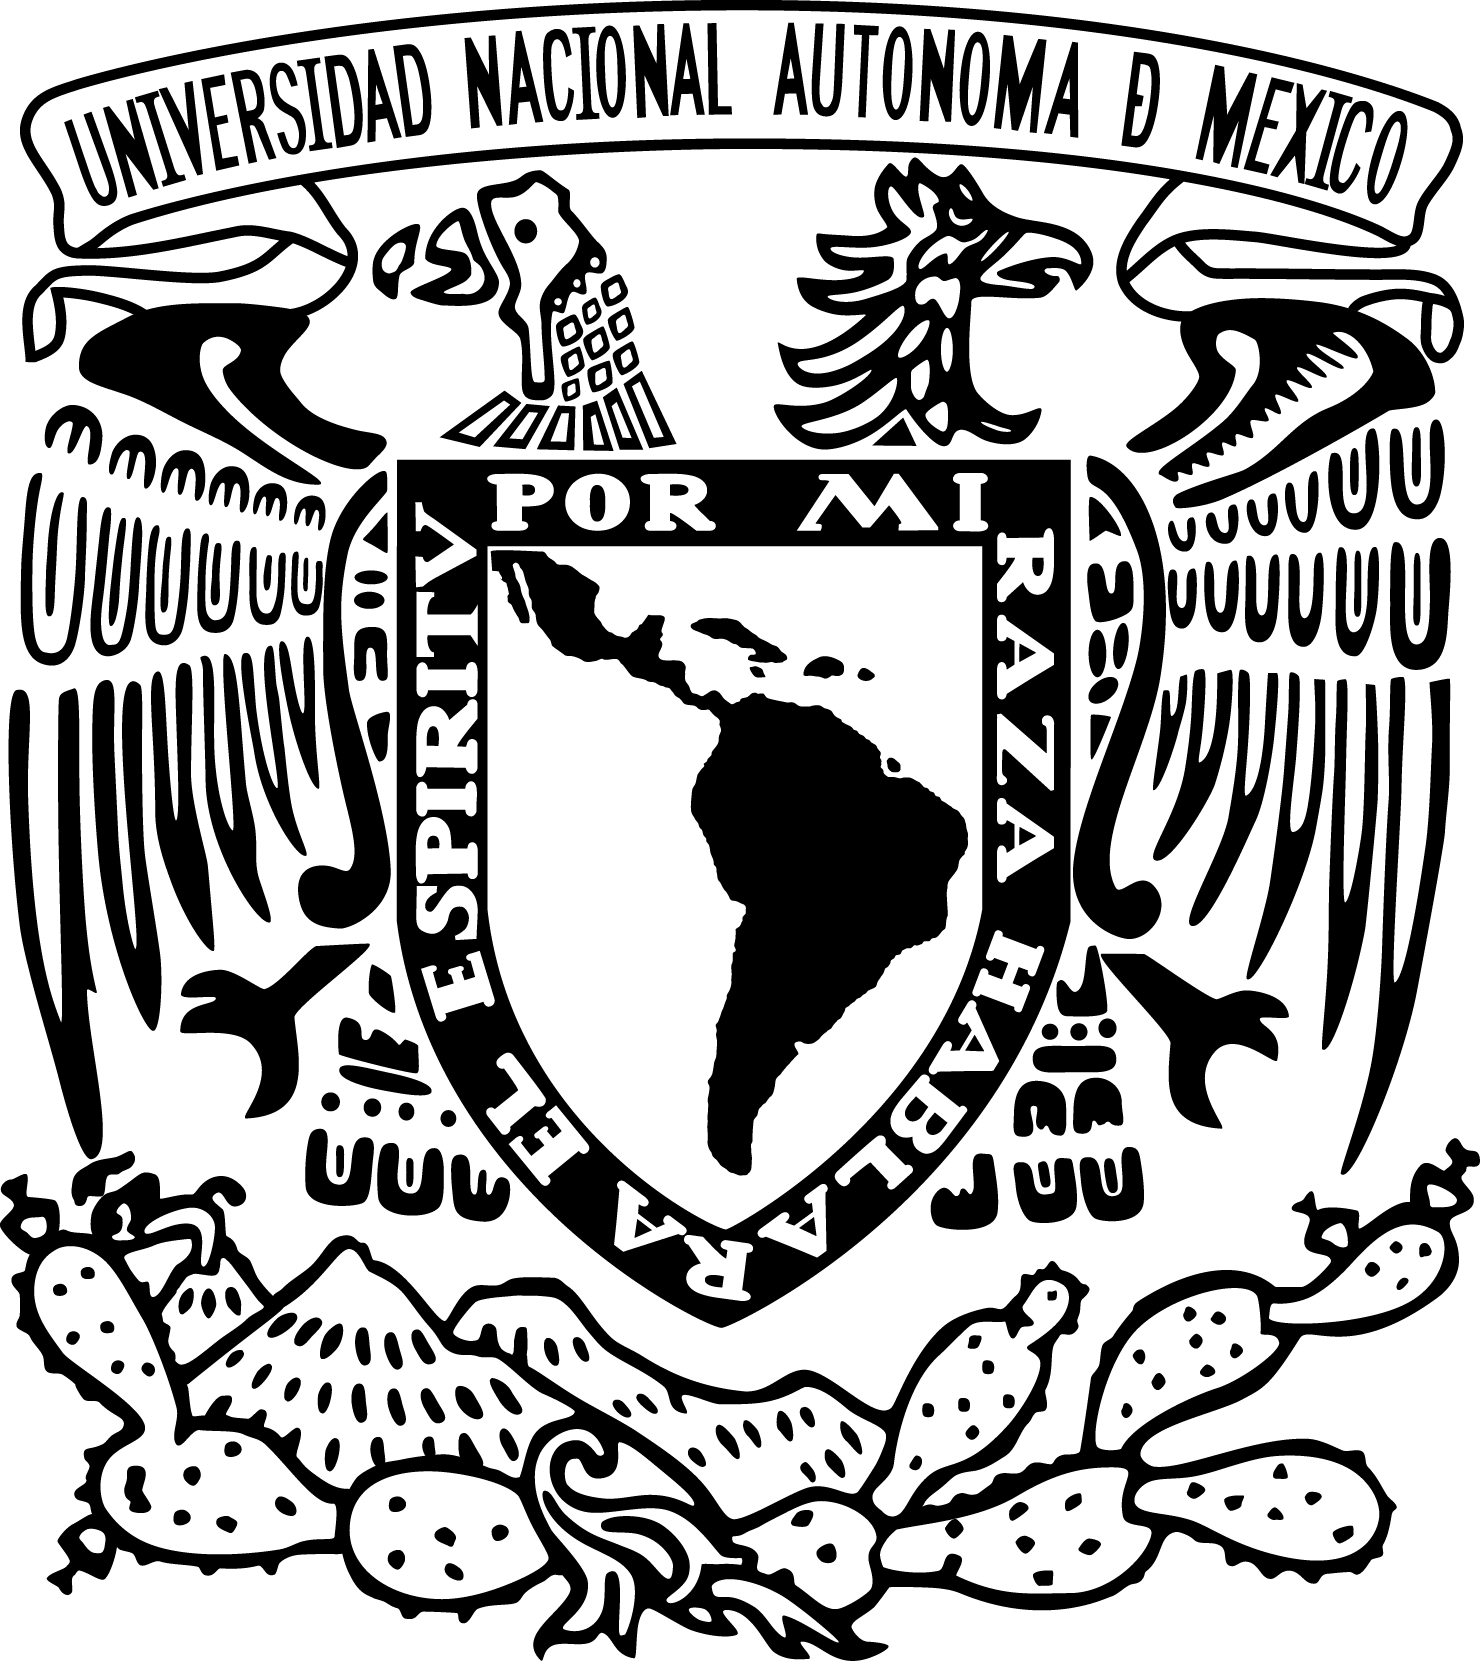
\includegraphics[width=0.3\textwidth]{unam-escudo}\vfill{}
  \Huge{Facultad de Ingeniería}\\
  \huge{Criptografía}\vfill{}
  \Huge{Proyecto Final}
  \\
  \vfill{}
  \LARGE{Alumnos:}
  \begin{flushleft}
    \begin{itemize}
      \item Machicao Cardoso Raúl Fernando
      \item Martínez López Andrés
      \item Romero Andrade Cristian
      \item Romero Andrade Vicente
    \end{itemize}
  \end{flushleft}
  \vfill{}
  % \Large{Grupo: 6}\\
  \Large{Semestre 2021--2}
  \vfill{}
  \LARGE{Profesora: Dra.~Rocio Alejandra Aldeco Perez}
  \vfill
  % \Large{Fecha de entrega: 14 de junio de 2021}
  % \vfill
  
\includegraphics[width=0.1\textwidth]{fi_logo}
\end{titlepage}


\title{Proyecto Final}
\author{
  \IEEEauthorblockN{
    Romero Andrade Cristian\IEEEauthorrefmark{1},
    Romero Andrade Vicente\IEEEauthorrefmark{2},
    Machicao Cardoso Raúl Fernando\IEEEauthorrefmark{3} y
    Martínez López Andrés\IEEEauthorrefmark{4}
  }
  \IEEEauthorblockA{Criptografía,
    Facultad de Ingeniería\\
    Email: \IEEEauthorrefmark{1}\href{mailto:cristian.romero@comunidad.unam.mx}{cristian.romero@comunidad.unam.mx},
    \IEEEauthorrefmark{2}\href{mailto:dark_reggae_93@comunidad.unam.mx}{dark\_reggae\_93@comunidad.unam.mx},
    \IEEEauthorrefmark{3}\href{mailto:laastar@comunidad.unam.mx}{laastar@comunidad.unam.mx},
    \IEEEauthorrefmark{4}\href{mailto:bockerlaila@comunidad.unam.mx}{bockerlaila@comunidad.unam.mx}}}

\maketitle{}

\tableofcontents{}

\subfile{./secciones/introduccion.tex}

\newpage{}

\subfile{./secciones/desarrollo.tex}

\newpage{}

\section{Conclusiones}\label{sec:concluciones}

Comparamos varios algoritmos, cada uno para una o unas tareas especificas, si bien
unos destacan en su velocidad, no cabe duda que pueden llegar a sacrificar robustes
(tal como pasó con SHA--1 en su momento). Unos algoritmos son más nuevos que otros, por
lo cual los más recientes tienen ciertos antecedentes que benefician para su diseño teniendo
una excelente relación velocidad---seguridad.

\nocite{*}

\newpage{}

\listoffigures{}
\listoftables{}
\listoflistings{}

\addcontentsline{toc}{section}{Referencias}
\printbibliography{}

\end{document}
